\documentclass[11pt,oneside,openany]{book}

\usepackage{graphicx}
\usepackage{color}    % to define macros for colors
\usepackage{listings} % package to include source code

\author{Matteo Franchin}

\title{Multiphysics~simulations of magnetic~nanostructures}

%TYPESETTING:----------------------------------------------------------

% Reset page margins properly for doublesided pages

% No headings
\pagestyle{plain}

% 1.5 interline spacing --> corresponds to linespread 1.3
% 2.0 interline spacing --> corresponds to linespread 1.6
\linespread{1.3}

\setlength{\marginparwidth}{0mm}
\setlength{\marginparsep}{0mm}
\setlength{\oddsidemargin}{0.7in} % corresponds to 1 + 0.7 = 1.7 inches
\setlength{\evensidemargin}{0.7in} % corresponds to 1.7 inches
\setlength{\textwidth}{145mm}
\setlength{\textheight}{220mm}
\setlength{\voffset}{-20mm}
\raggedbottom

%----------------------------------------------------------------------
% Extra colors

\definecolor{lightgrey}{cmyk}{0.05,0.05,0.05,0}
\definecolor{gray}{rgb}{0.5,0.5,0.5}

%----------------------------------------------------------------------
% Style for code listings

\lstdefinestyle{defaultstyle}{}
\lstset{language=Python}
\lstset{basicstyle=\ttfamily\scriptsize}
\lstset{showstringspaces=false}
\lstset{keywordstyle=\color{blue}}
\lstset{stringstyle=\color{red}}
\lstset{commentstyle=\color{gray}\emph}
\lstset{numbers=left,frame=single}
\lstset{backgroundcolor=\color{lightgrey}}

\begin{document}

\titlepage

\section{Example: bilayer film (strongly exchange coupled)}
Here is the example.

\begin{figure}[t]
\begin{center}
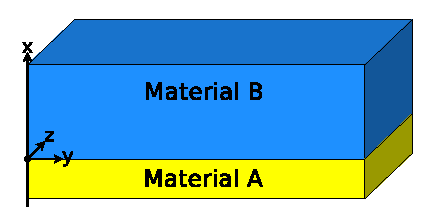
\includegraphics[width=10.0cm]{sketch}
\caption[Sketch]{A sketch of the system simulated in the script.}
\label{fig_es_types}
\end{center}
\end{figure}


\begin{figure}[!p]
\lstinputlisting[linerange=1-41]{spatially.py}
\caption{Part 1.}
\end{figure}

\begin{figure}[!p]
\lstinputlisting[linerange=42-84,firstnumber=42]{spatially.py}
\caption{Part 2.}
\end{figure}

\begin{figure}[!p]
\lstinputlisting[linerange=85-126,firstnumber=85]{spatially.py}
\caption{Part 3.}
\end{figure}

\end{document}
